\section{Оптимальные результаты для игрока С}

Теперь рассмотрим игру с точки зрения игрока С. Для каждой пары параметров $(\hat\mu, \hat\lambda)$ найдём
множество соответсвующих оптимальных пар $(p^*(\hat\mu, \hat\lambda), q^*(\hat\mu, \hat\lambda))$. Далее 
найдём значение свёртки для игрока С в этих точка:
$$
M(p^*,q^*,\hat\mu)=p^*\min{\{\dfrac{q^*}{\hat\mu};\dfrac{1-q^*}{2(1-\hat\mu)}\}} +
				   (1-p^*)\min\{\dfrac{q^*}{2\hat\mu};\dfrac{1-q^*}{1-\hat\mu}\}
$$
И изобразим множество значений функции в этих точках.
 
Рассмотрим все возможные сочетания значений для $p^*$ и $q^*$ в системах (7) и (8), что даст нам 6 следующих систем:

Напомню, что переменные имеют следующих области ограничений:
\[
p \in [0, 1],\quad q \in [0, 1],\quad
\mu \in [0, 1],\quad \lambda \in [0, 1]
\]

%---------------------------1------------------------
\textbf{(1)}

$$
	\begin{cases}
		p^* = 0 \\
		q^* = \dfrac{\mu}{2 - \mu} \\
		q^* > 1 - \lambda \\
		p^* + \mu - 1 \geqslant 0 \\
	\end{cases}
	\quad \sim \quad
	\begin{cases}
		p^* = 0 \\
		q^* = \dfrac{\mu}{2 - \mu} \\
		\dfrac{\mu}{2 - \mu} > 1 - \lambda \\
		\mu \geqslant 1 \quad \Rightarrow \quad \mu = 1 \\
	\end{cases}
	\quad \sim \quad
	\begin{cases}
		p^* = 0 \\
		q^* = 1 \\
		\lambda > 0 \\
		\mu = 1
	\end{cases}
$$

Значит при $\mu = 1, \lambda \in (0,1]$ имеем следующие оптимальные пары
$
\begin{cases}
	p^* = 0 \\ 
	q^* = 1 
\end{cases}
$

%---------------------------2------------------------
\textbf{(2)}

$$
	\begin{cases}
		p^* = 0 \\
		q^* = \dfrac{2 \mu}{1 + \mu} \\
		q^* > 1 - \lambda \\
		p^* + \mu - 1 \leqslant 0 \\
	\end{cases}
	\quad \sim \quad
	\begin{cases}
		p^* = 0 \\
		q^* = \dfrac{2\mu}{1 + \mu} \\
		\dfrac{2\mu}{1 + \mu} > 1 - \lambda \\
		\mu \leqslant 1
	\end{cases}
	\quad \sim \quad
	\begin{cases}
		p^* = 0 \\
		q^* = \dfrac{2 \mu}{1 + \mu} \\
		\lambda > \dfrac{1 - \mu}{1 + \mu} \\
		\mu \leqslant 1
	\end{cases}
$$

Значит при $\mu \in [0, 1], \lambda \in (\dfrac{1 - \mu}{1 + \mu}, 1]$
имеем следующие оптимальные пары
$
\begin{cases}
	p^* = 0 \\
	q^* = \dfrac{2\mu}{1 + \mu} 
\end{cases}
$



%---------------------------3------------------------
\textbf{(3)}

$$
	\begin{cases}
		p^* = 1 \\
		q^* = \dfrac{\mu}{2 - \mu} \\
		q^* < 1 - \lambda \\
		p^* + \mu - 1 \geqslant 0 \\
	\end{cases}
	\quad \sim \quad
	\begin{cases}
		p^* = 1 \\
		q^* = \dfrac{\mu}{2 - \mu} \\
		\dfrac{\mu}{2 - \mu} < 1 - \lambda \\
		\mu \geqslant 0
	\end{cases}
	\quad \sim \quad
	\begin{cases}
		p^* = 1 \\
		q^* = \dfrac{\mu}{2 - \mu} \\
		\lambda < 2\dfrac{1 - \mu}{2 - \mu} \\
		\mu \geqslant 0
	\end{cases}
$$

Значит при $\mu \in [0, 1], \lambda \in [0, 2\dfrac{1 - \mu}{2 - \mu})$
имеем следующие оптимальные пары
$\begin{cases}
	p^* = 1 \\
	q^* = \dfrac{\mu}{2 - \mu}
\end{cases}$

%---------------------------4------------------------
\textbf{(4)}

$$
	\begin{cases}
		p^* = 1 \\
		q^* = \dfrac{2\mu}{1 + \mu} \\
		q^* < 1 - \lambda \\
		p^* + \mu - 1 \leqslant 0 \\
	\end{cases}
	\quad \sim \quad
	\begin{cases}
		p^* = 1 \\
		q^* = \dfrac{2\mu}{1 + \mu} \\
		\dfrac{2\mu}{1 + \mu} < 1 - \lambda \\
		\mu \leqslant 0 \quad \Rightarrow \quad \mu = 0 \\
	\end{cases}
	\quad \sim \quad
	\begin{cases}
		p^* = 1 \\
		q^* = 0 \\
		\lambda < 1 \\
		\mu = 0
	\end{cases}
$$

Значит при $\mu=0, \lambda \in [0, 1)$ имеем следующие оптимальные пары
$\begin{cases}
	p^* = 1 \\
	q^* = 0 
\end{cases}$

%---------------------------5------------------------
\textbf{(5)}

$$
	\begin{cases}
		p^* \in [0, 1] \\
		q^* = \dfrac{\mu}{2 - \mu} \\
		q^* = 1 - \lambda \\
		p^* + \mu - 1 \geqslant 0 \\
	\end{cases}
	\quad \sim \quad
	\begin{cases}
		p^* \in [0, 1] \\
		q^* = \dfrac{\mu}{2 - \mu} \\
		\dfrac{\mu}{2 - \mu} = 1 - \lambda \\
		p^* \geqslant 1 - \mu \\
	\end{cases}
	\quad \sim \quad
	\begin{cases}
		p^* \in [1 - \mu, 1] \\
		q^* = \dfrac{\mu}{2 - \mu} \\
		\lambda = 2\dfrac{1 - \mu}{2 - \mu} \\
	\end{cases}
$$

Значит при $\lambda = 2\dfrac{1 - \mu}{2 - \mu}, \mu \in [0, 1]$ 
имеем следующие оптимальные пары
$
	\begin{cases}
		p^* \in [1 - \mu, 1] \\
		q^* = \dfrac{\mu}{2 - \mu}
	\end{cases}
$

%---------------------------6------------------------
\textbf{(6)}

$$
	\begin{cases}
		p^* \in [0, 1] \\
		q^*= \dfrac{2\mu}{1 + \mu} \\
		q^* = 1 - \lambda \\
		p^* + \mu - 1 \leqslant 0 \\
	\end{cases}
	\quad \sim \quad
	\begin{cases}
		p^* \in [0, 1] \\
		q^* = \dfrac{2\mu}{1 + \mu} \\
		\dfrac{2\mu}{1 + \mu} = 1 - \lambda \\
		p^* \leqslant 1 - \mu 
	\end{cases}
	\quad \sim \quad
	\begin{cases}
		p^* \in [0, 1 - \mu] \\
		q^* = \dfrac{2\mu}{1 + \mu} \\
		\lambda = \dfrac{1 - \mu}{1 + \mu} \\
	\end{cases}
$$

Значит при $\mu \in [0, 1], \lambda = \dfrac{1 - \mu}{1 + \mu}$
имеем следующие оптимальные пары
$
	\begin{cases}
		p^* \in [0, 1 - \mu] \\
		q^* = \dfrac{2\mu}{1 + \mu} \\
	\end{cases}
$

Теперь на квадрате $(p, q) \in [0, 1]^2$ рассмотрим все области,
в которых множества оптимальных пар постоянны. 
И найдём множества значений функции 

$$
	\overline G(p, q, \mu)=
	p \min \{
		\dfrac{q}{\mu};
		\dfrac{1-q}{2(1-\mu)}
	\} + (1 - p) \min \{
		\dfrac{q}{2\mu};
		\dfrac{1 - q}{1 - \mu}
	\},
$$

В этих областях

\begin{center}
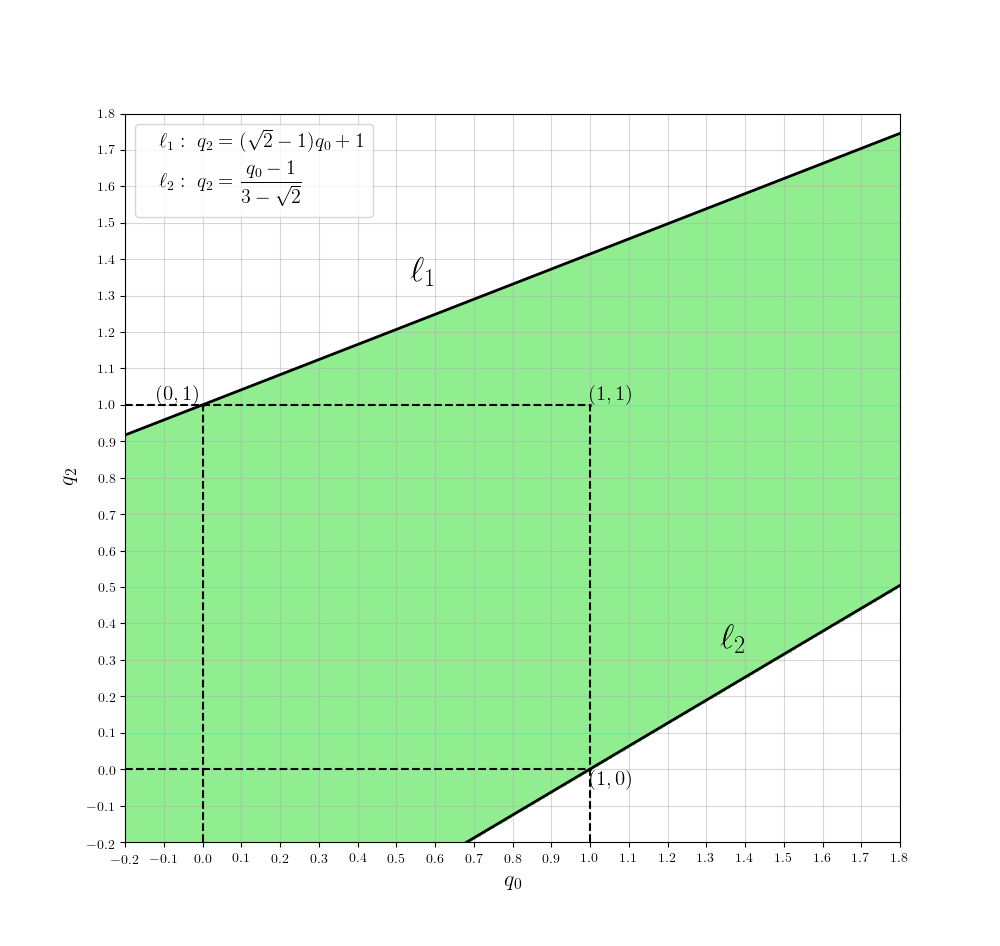
\includegraphics[scale=0.4]{part_2/graf_3_1}
\end{center}

1) $\mu = 0, \lambda \in [0, 1)$: 
$
	\begin{cases}
		p^* = 1 \\ 
		q^* = 0 
	\end{cases};
	\begin{cases}
		p^* = 1 \\
		q^* = \dfrac{\mu}{2 - \mu} = \{\mu = 0 \} = 0
	\end{cases}
$ 

\hfill \break

Получаем множества оптимальных стратегий 

$(P^* \times Q^*) = (\{1\} \times \{0\})$, где $\times$ - это декартово 
произведение, тогда

$$\overline G(1, 0, 0) = \dfrac{1}{2}$$

\begin{center}
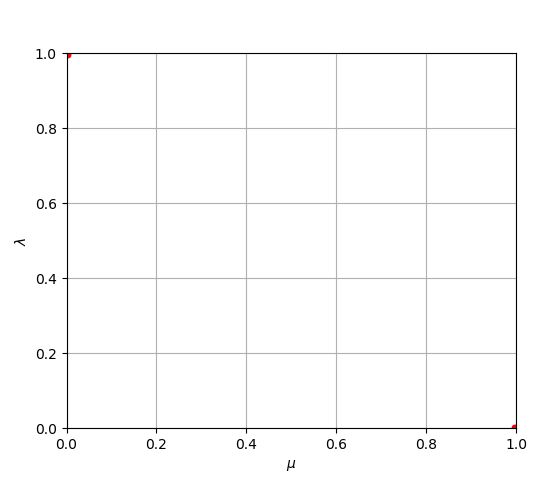
\includegraphics[scale=0.7]{part_2/graf_3_2}
\end{center}


2.1) $\mu=0, \lambda =1$: 
$
	\begin{cases}
		p^* \geqslant 1 - \mu = \{\mu = 0\} = 1 \\
		q^* = \dfrac{\mu}{2 - \mu} = \{\mu = 0\} = 0
	\end{cases};
	\begin{cases}
		p^* \leqslant 1 - \mu = \{\mu = 0\} = 1 \\
		q^* = \dfrac{2\mu}{1 + \mu} = \{\mu = 0\} = 0 
	\end{cases}
$

\hfill \break 
Получаем множества оптимальных стратегий 
$(P^* \times Q^*) = ([0, 1] \times \{0\})$ тогда
$$\overline G([0, 1], 0, 0) = [0.5, 1]$$
%\vspace{5mm}

2.2) $\mu = 1, \lambda = 0$: 
$
	\begin{cases}
		p^* \geqslant 1-\mu = \{\mu=1\}=0 \\
		q^* = \dfrac{\mu}{2-\mu} = \{\mu=1\}=1
	\end{cases} ;
	\begin{cases}
		p^* \leqslant 1 - \mu = \{\mu = 1\} = 0\ \\
		q^* = \dfrac{2\mu}{1 + \mu} = \{\mu = 1\} = 1 
	\end{cases}
$

\hfill \break 
Получаем множества оптимальных стратегий 
$(P^* \times Q^*) = ([0, 1] \times \{1\})$ тогда
$$\overline G([0, 1], 1, 1) = [0.5, 1]$$

\begin{center}
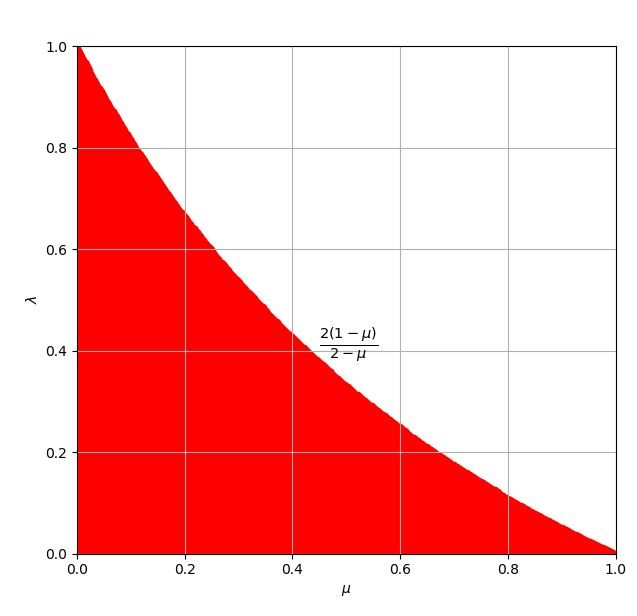
\includegraphics[scale=0.6]{part_2/graf_3_3}
\end{center}


3) $\mu \in (0,1), \lambda \in (0, \dfrac{1 - \mu}{1 + \mu}]$: 
$
	\begin{cases}
		p^* = 1 \\ 
		q^* = \dfrac{\mu}{2 - \mu} 
	\end{cases}
$

\hfill \break
Получаем множества оптимальных стратегий 
$(P^* \times Q^*) = (\{1\} \times \{\dfrac{\mu}{2 - \mu}\})$ тогда
$$
	\overline G(1, \dfrac{\mu}{2 - \mu}, \mu)=
	\min \big\{
		\dfrac{\mu}{2 - \mu}; 
		\dfrac{1 - \dfrac{\mu}{2 - \mu}}{2(1 - \mu)}
	\big\}
	=\dfrac{1}{2 - \mu}
$$

\begin{center}
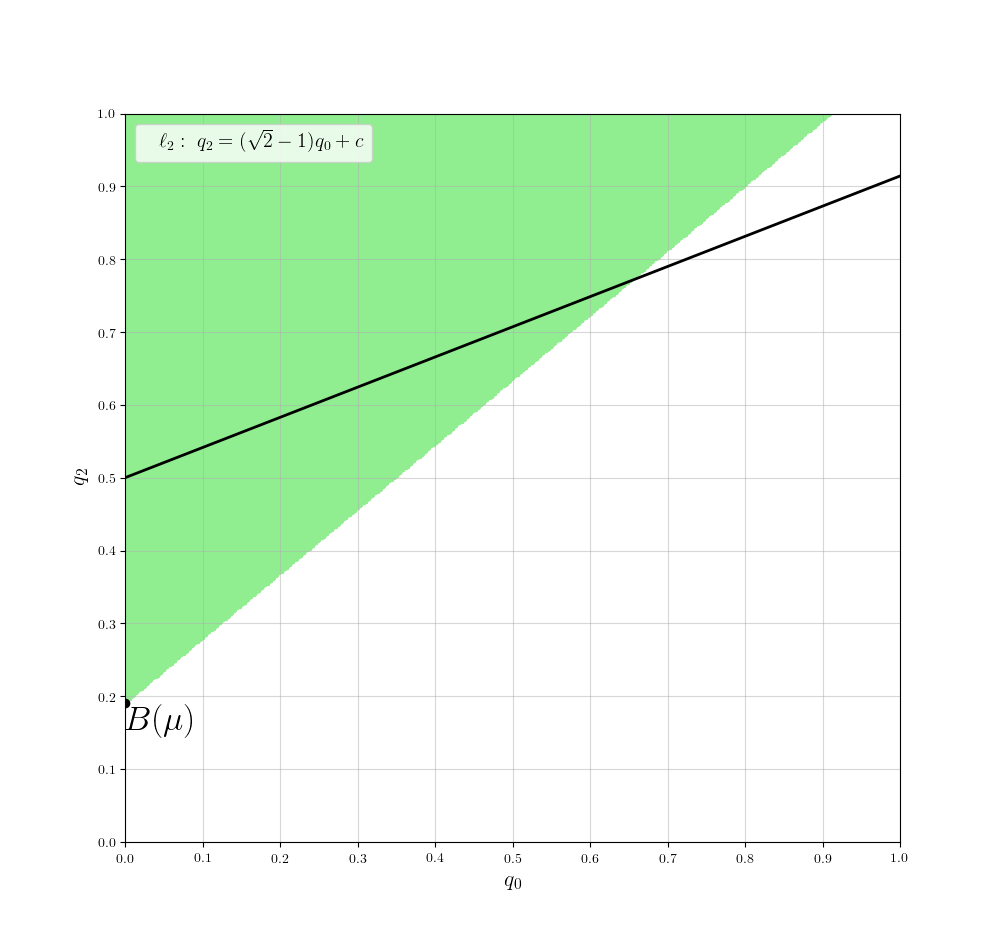
\includegraphics[scale=0.6]{part_2/graf_3_4}
\end{center}


4) $\mu \in (0,1), \lambda = \dfrac{1 - \mu}{1 + \mu}$:
$
	\begin{cases}
		p^* \in [0, 1 - \mu] \cup \{1\} \\
		q^* = \dfrac{\mu}{2 - \mu}
	\end{cases}
$

\hfill \break

4.1) Получаем множества оптимальных стратегий 
$(P^* \times Q^*) = (\{1\} \times \{\dfrac{\mu}{2 - \mu}\})$ тогда
$$
	\overline G(1,\dfrac{\mu}{2-\mu},\mu)=\dfrac{1}{2-\mu}
$$

4.2) Получаем множества оптимальных стратегий 
$(P^* \times Q^*) =([0,1-\mu] \times \{\dfrac{2\mu}{1+\mu}\})$ тогда
$$
	\overline G(p,\dfrac{2\mu}{1+\mu},\mu) =
	p\dfrac{1}{2(1 + \mu)} + (1 - p)\dfrac{1}{1 + \mu}=
	\dfrac{2 - p}{2(1 + \mu)} \geqslant
	\dfrac{2 - (1 - \mu)}{2(1 + \mu)} =
	\dfrac{1 + \mu}{2(1 + \mu)} =
	\dfrac{1}{2}
$$
$$
	\overline G(p, \dfrac{2\mu}{1 + \mu}, \mu) \leqslant 
	\dfrac{1}{1 + \mu} \Rightarrow
	\overline G (p, \dfrac{2\mu}{1 + \mu}, \mu) = 
	[0.5, 	\dfrac{1}{1 + \mu}]
$$

\begin{center}
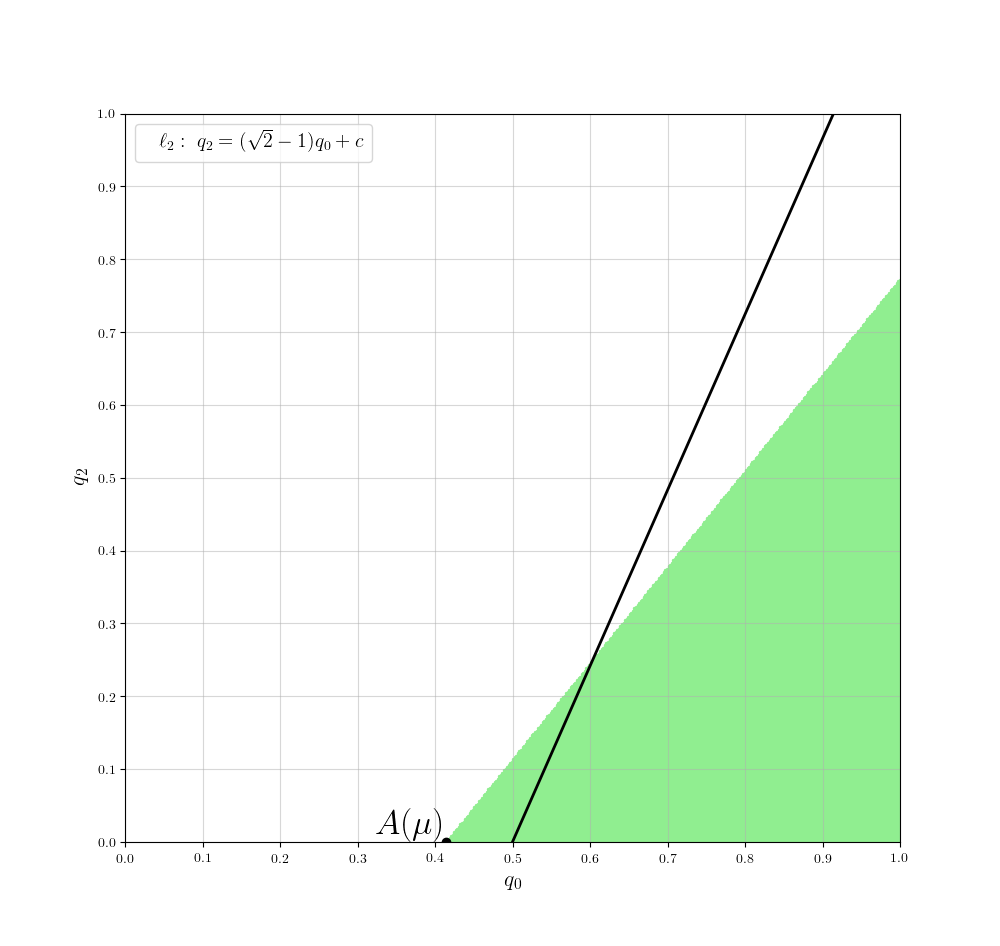
\includegraphics[scale=0.5]{part_2/graf_3_5}
\end{center}


5) $\mu \in [(, 1), \lambda \in 
[0, 2\dfrac{1 - \mu}{2 - \mu}] \cap (\dfrac{1 - \mu}{1 + \mu}, 1]$: 
$
	\begin{cases}
		p^* = 0 \\
		q^* = \dfrac{2\mu}{1 + \mu}
	\end{cases};
	\begin{cases}
		p^* = 1 \\
		q^* = \dfrac{\mu}{2 - \mu}
	\end{cases}
$

\hfill \break

5.1) Получаем множества оптимальных стратегий 
$(P^* \times Q^*) = (\{0\} \times \{\dfrac{2\mu}{1 + \mu}\})$ тогда
$$
	\overline G(0, \dfrac{2\mu}{1 + \mu}, \mu) = \dfrac{1}{1 + \mu}
$$

5.2) Получаем множества оптимальных стратегий 
$(P^* \times Q^*) =(\{1\}\times \{\dfrac{\mu}{2 - \mu}\})$ тогда
$$
	\overline G(1, \dfrac{\mu}{2 - \mu}, \mu) = \dfrac{1}{2 - \mu}
$$

\begin{center}
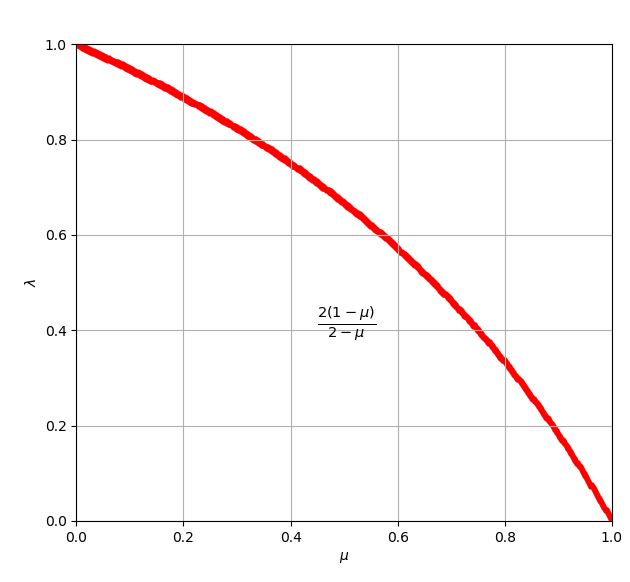
\includegraphics[scale=0.5]{part_2/graf_3_6}
\end{center}

6) $\mu \in (0, 1), \lambda = 2\dfrac{1 - \mu}{2 - \mu}$: 
$
	\begin{cases}
		p^* = 0 \\
		q^* = \dfrac{2\mu}{1 + \mu}
	\end{cases};
	\begin{cases}
		p^* \in [0, 1 - \mu] \\
		q^* = \dfrac{\mu}{2 - \mu} 
	\end{cases}
$

\hfill \break
6.1) Получаем множества оптимальных стратегий 
$(P^* \times Q^*) =(\{0\} \times \{\dfrac{2\mu}{1 + \mu}\})$ тогда
$$
	\overline G(0, \dfrac{2\mu}{1 + \mu}, \mu) = \dfrac{1}{1 + \mu}
$$
6.2) Получаем множествo оптимальных стратегий 
$(P^* \times Q^*) =([1 - \mu, 1] \times \{\dfrac{\mu}{2 - \mu}\})$ тогда
$$
	\overline G(p, \dfrac{\mu}{2 - \mu}, \mu) =
	p\dfrac{1}{2 - \mu} + (1 - p)\dfrac{1}{2(2 - \mu)} =
	\dfrac{1 + p}{2(2 - \mu)} \geqslant \dfrac{2 - \mu}{2(2 - \mu)} =
	\dfrac{1}{2}
$$
$$
	\overline G(p, \dfrac{\mu}{2 - \mu}, \mu) \leqslant
 	\dfrac{1}{2 - \mu} \Rightarrow \overline G(p, \dfrac{\mu}{2 - \mu}, \mu) =
 	[0.5, \dfrac{1}{2 - \mu}]
$$

\begin{center}
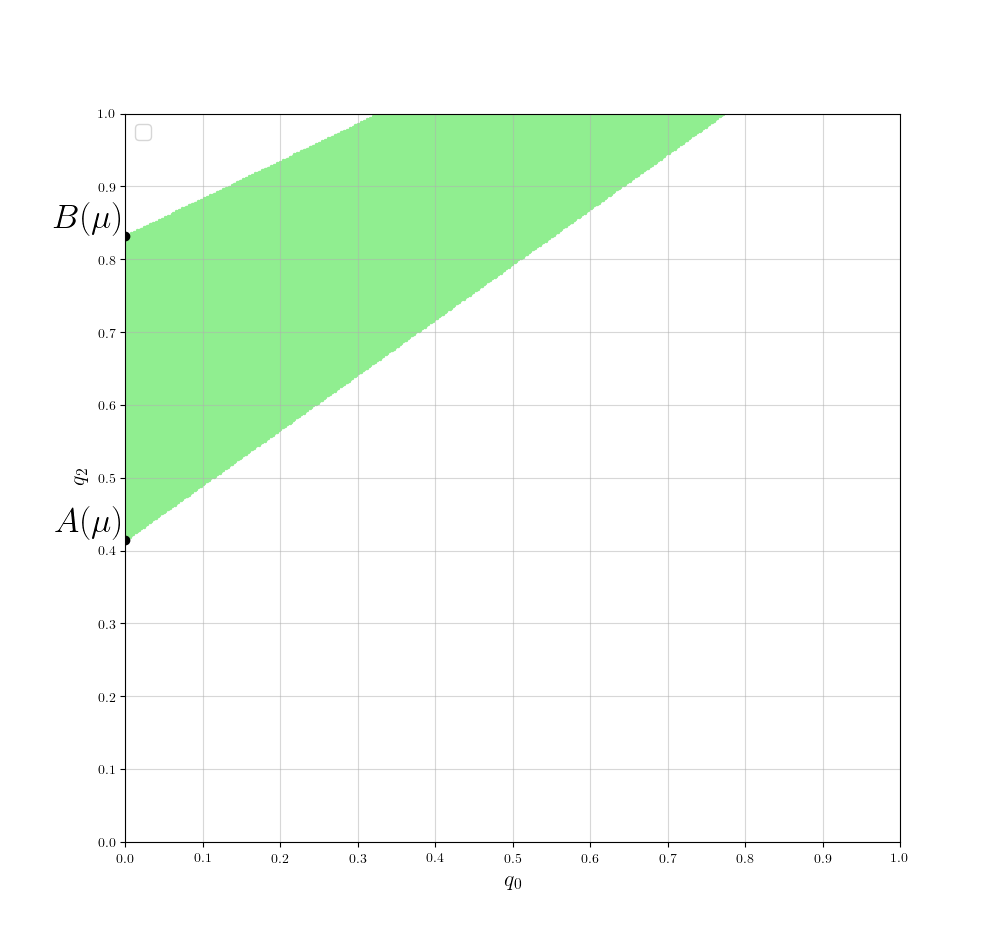
\includegraphics[scale=0.5]{part_2/graf_3_7}ntheorem
\end{center}

7) $\mu \in (0, 1), \lambda \in (2\dfrac{1 - \mu}{2 - \mu}, 1]$: 
$
	\begin{cases}
		p^* = 0 \\
		q^* = \dfrac{2\mu}{1 + \mu}
	\end{cases}
$

\hfill \break

Получаем множества оптимальных стратегий 
$(P^* \times Q^*) =(\{0\} \times \{\dfrac{2\mu}{1 + \mu}\})$ тогда

$$
	\overline G(0, \dfrac{2\mu}{1 + \mu}, \mu)=
	\min \big\{
		\dfrac{1}{\mu}\dfrac{2\mu}{1 + \mu}; 
		\dfrac{1 - \dfrac{2\mu}{1 + \mu}}{1 - \mu}
	\big\} =
	\dfrac{1}{1 + \mu}
$$

\begin{center}
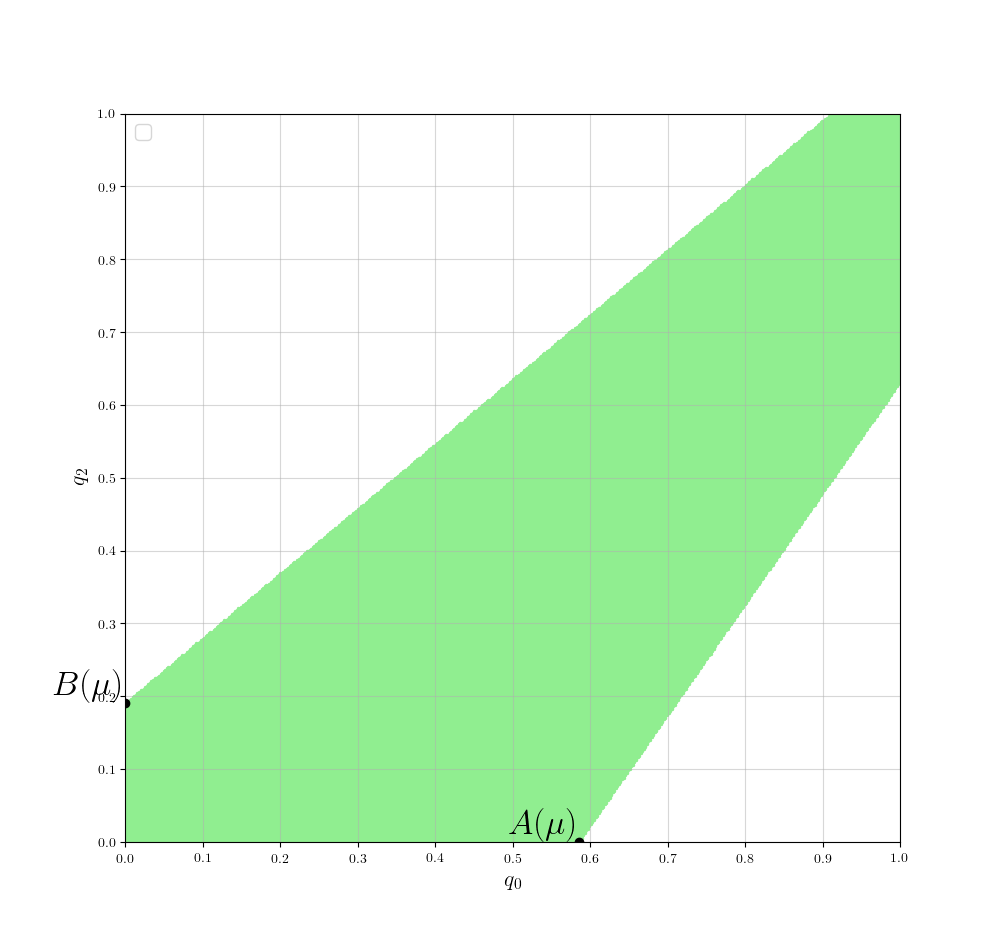
\includegraphics[scale=0.5]{part_2/graf_3_8}
\end{center}

8) $\mu = 1, \lambda \in (0, 1] $: 
$
	\begin{cases}
		p^* = 0 \\
		q^* = 1 \\
	\end{cases};
	\begin{cases}
		p^* = 0 \\
		q^* = \dfrac{2\mu}{1 + \mu} = \{\mu = 1\} = 1 \\
	\end{cases}
$

\hfill \break
Получаем множества оптимальных стратегий 
$(P^* \times Q^*) =(\{0\} \times \{1\})$ тогда
$$
	\overline G(0, 1, 1) = \dfrac{1}{2}
$$
\vspace{40mm}

Теперь на квадрате $(\mu, \lambda) \in [0, 1]^2$ мы рассмотрели все точки
и для каждой нашли оптимальные пары $p^*(\mu, \lambda)$
и $q^*(\mu, \lambda)$ и соответсвующие значения функции 
$M(p^*(\mu, \lambda),q^*(\mu, \lambda),\mu)$. Далее на квадрате
$[0, 1]^{2}$ изобразим все точки, которые принимает вектор $(\mu M(p^*,q^*,\mu), (1-\mu) M(p^*,q^*,\mu))$ при
$(\mu, \lambda)\in[0, 1]^{2}$

\begin{center}
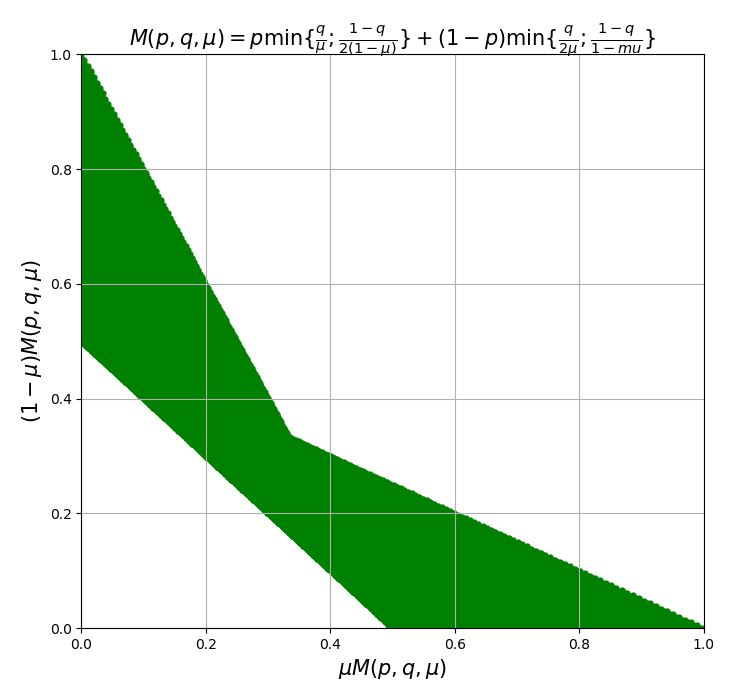
\includegraphics[scale=0.6]{part_2/graf_4}
\end{center}

Поясним график: \\
нижняя огибающая в координатах $X,Y$: $y=\dfrac{1}{2}-x$, \\
верхняя огибающая в координатах $X,Y$: 
$y=
\begin{cases}
	1 - 2x, & x \in [0, \dfrac{1}{3}) \\
	\dfrac{1 - x}{2}, & x \in [\dfrac{1}{3}, 1]
\end{cases}.
$
